27. \begin{figure}[ht!]
\center{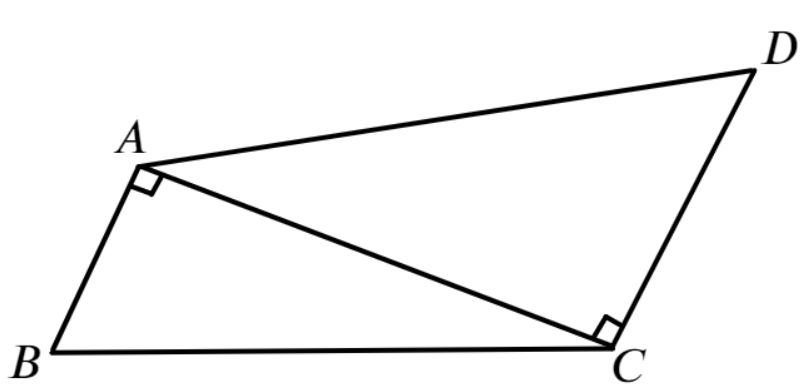
\includegraphics[scale=0.35]{g8-27.png}}
\end{figure}\\
Так как $5^2+12^2=13^2$ и $9^2+12^2=15^2,$ по обратной теореме Пифагора треугольники $ABC$ и $CAD$ являются прямоугольными. Тогда $S_{ABCD}=S_{ABC}+S_{CAD}=\cfrac{1}{2}\cdot5\cdot12+\cfrac{1}{2}\cdot9\cdot12=84.$\\
